\chapter{\label{ch:michel}Study of Michel Electrons in \protodune{}} 

\minitoc

%%%%%%%%%%%%%%%%%%%%%%%%%%%%%%%%%%%%%%%%%%%%%%%%%%%%%%%%%%%%%%%%%%%%%%%%%%%%%%%%
% FROM COS
%
% This chapter will cover the primary analysis of this thesis; a study of Michel
% electrons in the ProtoDUNE--SP detector which aims to investigate the agreement
% between data and simulation, and to provide an estimate of the energy scale
% uncertainty and energy scale bias for electrons in the 0--60 MeV range. 
% 
% The work done for this section is ongoing; preliminary work on this topic was
% presented in the report submitted for transfer of status. The rest of the work
% for this section is expected to be completed by the end of October 2019.
% 
% \noindent The work done as of writing for this chapter is as follows:
% \begin{itemize}[noitemsep,nolistsep]
% 	\item Event selection algorithm developed based on clustering of the Michel
% 	like hits discussed in the previous chapter.
% 	\begin{itemize}[noitemsep,nolistsep]
% 		\item Purity of > 98\% and efficiency of 5\% measured in ProtoDUNE--SP 
% 		simulations.
% 	\end{itemize}
% 	\item Two possible energy reconstruction algorithms developed.
% 	\begin{itemize}[noitemsep,nolistsep]
% 		\item Cone algorithm.
% 		\item Semantic segmentation algorithm with U-ResNet CNN architecture.
% 	\end{itemize}
% \end{itemize}
% 
% \noindent The work left to do is as follows:
% \begin{itemize}[noitemsep, nolistsep]
% 	\item Validation of algorithms on the real ProtoDUNE--SP data.
% 	\item Data MC comparison for Michel electron energy spectrum.
% 	\item Energy scale uncertainty and energy scale bias measurements with 
% 	measured Michel electron energy spectrum.
% \end{itemize}
% 
% \noindent An example Michel electron candidate event from the real ProtoDUNE--SP 
% data is given in figure \ref{fig:michel_event}.
% 
% \begin{figure}[h]
% 	\centering
% 	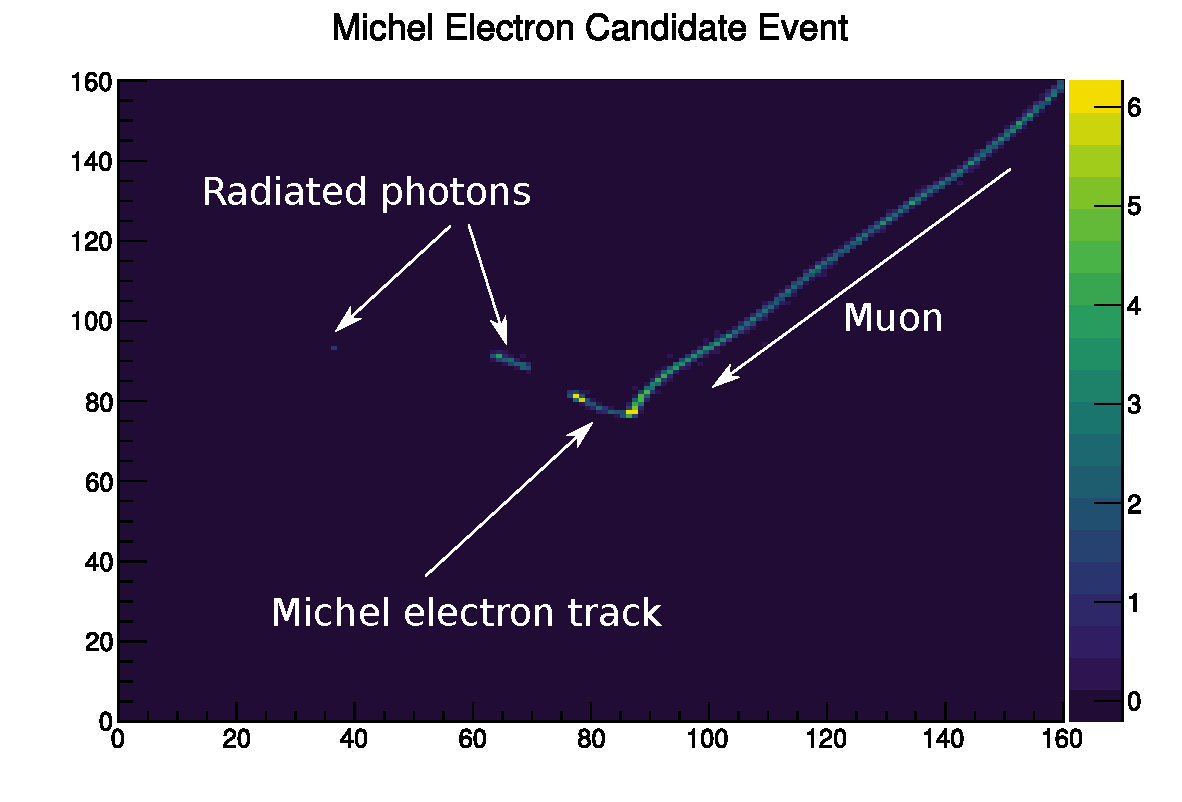
\includegraphics[width=0.7\textwidth]{figures/michel_candidate.pdf}
% 	\caption[Michel electron candidate event from ProtoDUNE--SP data.]{Michel 
% 	electron candidate event from ProtoDUNE--SP data.}
% 	\label{fig:michel_event}
% \end{figure}
%
%%%%%%%%%%%%%%%%%%%%%%%%%%%%%%%%%%%%%%%%%%%%%%%%%%%%%%%%%%%%%%%%%%%%%%%%%%%%%%%%
\noindent
Studying electrons in the tens of MeV energy range can provide valuable input 
into reconstruction techniques and energy uncertainty for the measurement of
astrophysical neutrinos from supernova bursts. Understanding the response of
LArTPC detectors to electrons in this range will be important for any large
scale LArTPC experiment wishing to study supernova bursts. At these energies
electron interactions have large contributions from both ionisation energy loss
and radiative energy loss and therefore they have a unique signature which is 
neither track--like or shower--like. Low--energy electrons therefore require 
unique reconstruction algorithms, to maximise the overall reconstruction 
performance. 

This chapter will discuss an approach to low--energy electron reconstruction 
in LArTPC detectors based on the use of convolutional neural networks and 
semantic segmentation. Michel electron events from \protodune{} will be used 
to test the performance of this technique and to provide an estimate of the 
energy uncertainty of LArTPC detectors for low--energy electrons.

In this chapter Section \ref{ME_LAr} will discuss the signature left by Michel
electrons in liquid argon, and the implications of this signature on
reconstructing Michel electron events in \protodune{}. This will be followed by
a discussion of the algorithm used to select Michel electron events in Section
\ref{ME_ES}. The Michel electron event reconstruction will be discussed in
Sections \ref{ME_R}. Finally, the results of this chapter and the implications
for the DUNE far detector will be summarised in Section \ref{ME_EU}.

\section{Michel Electrons in Liquid Argon} \label{ME_LAr}
Michel electrons are produced when a muon decays at rest. In vacuum, this 
decay gives rise to a characteristic energy spectrum which has a sharp 
cut--off at around 50 MeV, corresponding to half the muon mass. In matter it 
is also possible for $\mu^-$ to be captured on nuclei before they decay, this 
causes a broadening of the Michel electron spectrum for these events. A 
comparison of the Michel electron energy spectrum for free $\mu^+$ and 
captured $\mu^-$ is given in Figure \ref{fig:michel_spec}. The capture process 
occurs roughly 70\% of the time for negative muons in liquid argon, therefore, 
in \protodune{} the observed Michel electron energy spectrum is a combination 
of the two processes in roughly equal quantities.
\begin{figure}

	\centering
	% TODO
	\begin{subfigure}[b]{0.48\textwidth}
		\centering
		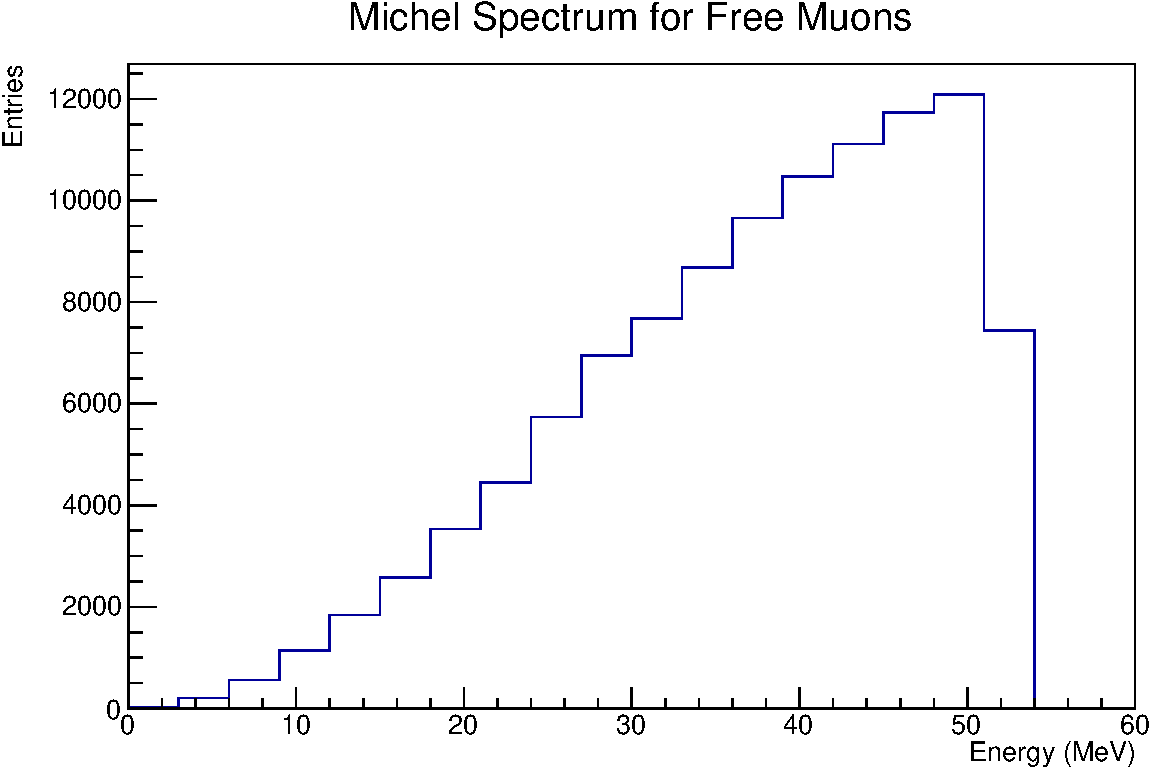
\includegraphics[width=\textwidth]{figures/michel_spec_free.pdf}
		\caption {Free Muons.}
		\label{fig:michel_spec_free}
	\end{subfigure}
	\hfill
	\begin{subfigure}[b]{0.48\textwidth}
		\centering
		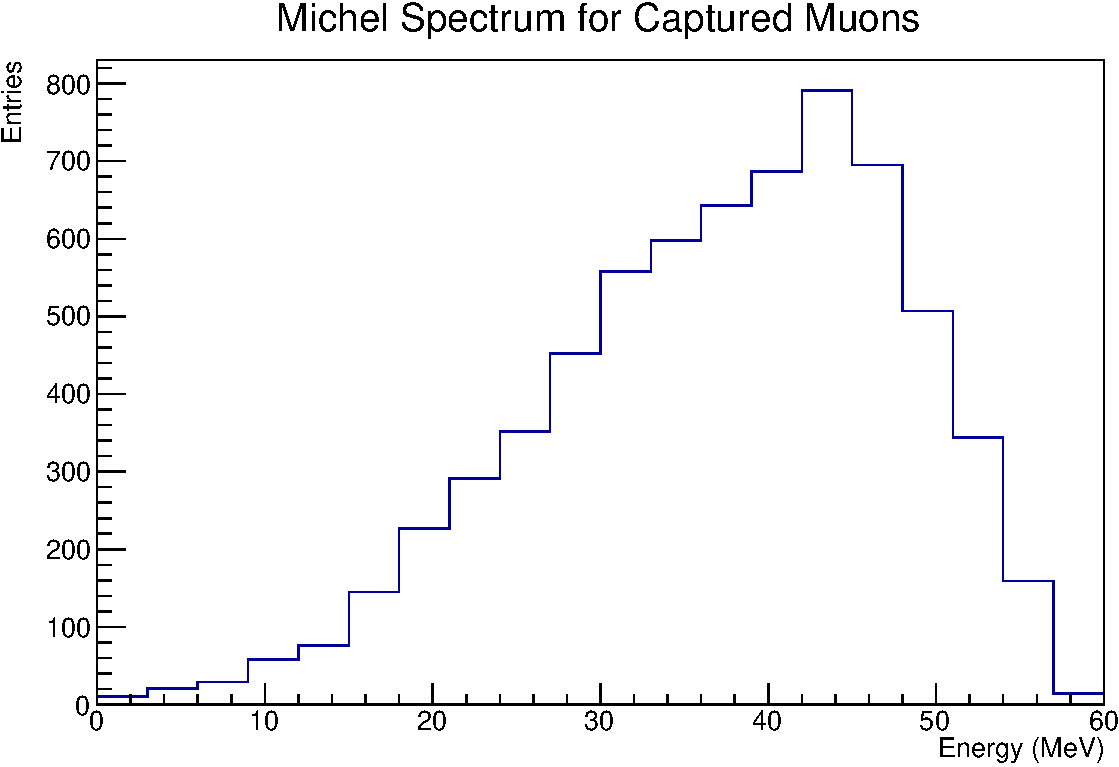
\includegraphics[width=\textwidth]{figures/michel_spec_cap.pdf}
		\caption {Captured Muons.}
		\label{fig:michel_spec_cap}
	\end{subfigure}

	\caption
	[Michel electron energy spectra in liquid argon.]
	{Michel electron energy spectra in liquid argon.}

	\label{fig:michel_spec}

\end{figure}

As discussed in chapter \ref{ch:energyloss}, the energy loss for electrons in
liquid argon passes from an ionisation dominated regime to a radiation dominated
regime in the tens of MeV region. The crossover point for this transition occurs
at around 45 MeV, very close to the peak of the Michel electron spectrum. This
leads to a unique signature for Michel electrons in liquid argon detectors, a
short ($\sim$ 5cm) track segment is surrounded by a number of small radiated 
energy deposits. Figure \ref{fig:michel_event} shows an example of a Michel 
electron candidate from \protodune{} data, along with labels of the key 
features.

\begin{figure}
	\centering
	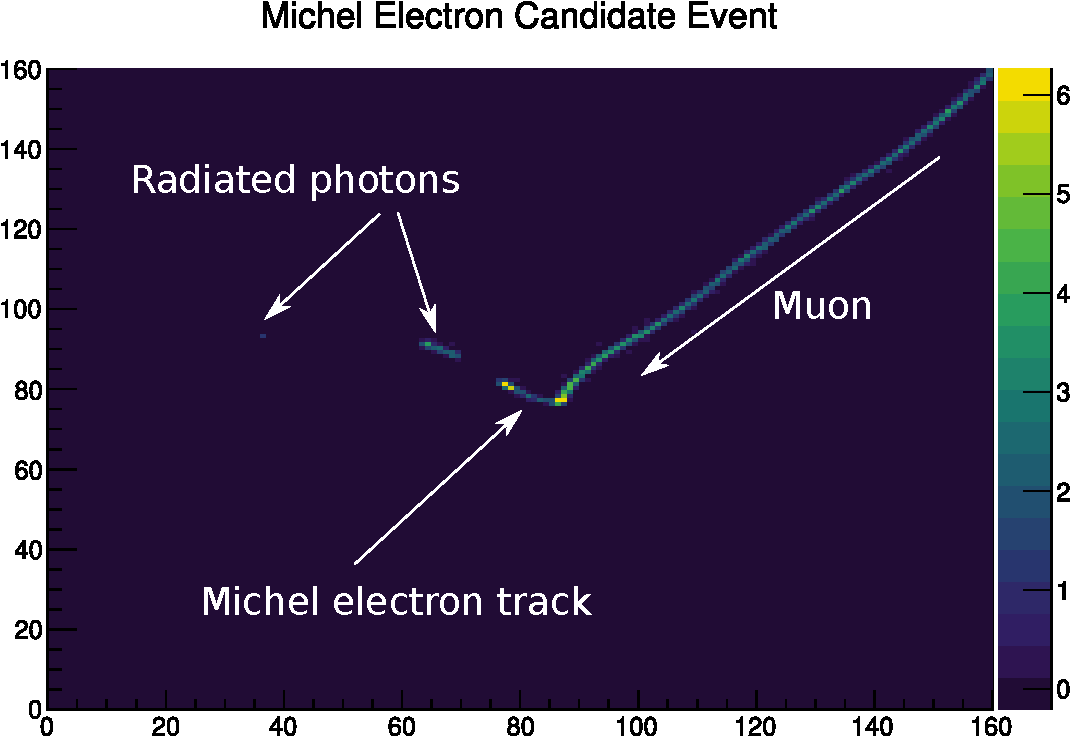
\includegraphics[width=\textwidth]{figures/michel_candidate_labelled.pdf}
	\caption
	[Michel electron candidate event from ProtoDUNE--SP data.]
	{Michel electron candidate event from ProtoDUNE--SP data.}
	\label{fig:michel_event}
\end{figure}

One of the main challenges for Michel electron reconstruction in liquid argon is
to successfully associate the radiated energy depositions back to the initial
Michel electron once they have produced ionisation in the detector. Photons have
a radiation length of around 20--30 cm in liquid argon which is many times
larger than the size of the typical track--like part of the event, around 5 cm. 
Figure \ref{fig:photon_spec} shows the spectrum of radiated photons from Michel 
electron events in \protodune{} simulation alongside the photon multiplicity 
as a function of Michel electron energy. While most of the radiated photons 
only carry a small fraction of the Michel electrons energy, in some cases a 
single radiated photon can carry a significant fraction of the electron 
energy. In addition, around the peak of the Michel electron spectrum ($\sim$
45 MeV) there is a high photon multiplicity and a large spread in the
multiplicity distribution. The combination of these effects leads to a
significant spread in the fraction of radiated energy for Michel electron
events.

\begin{figure}

	\centering

	\begin{subfigure}[b]{\textwidth}
		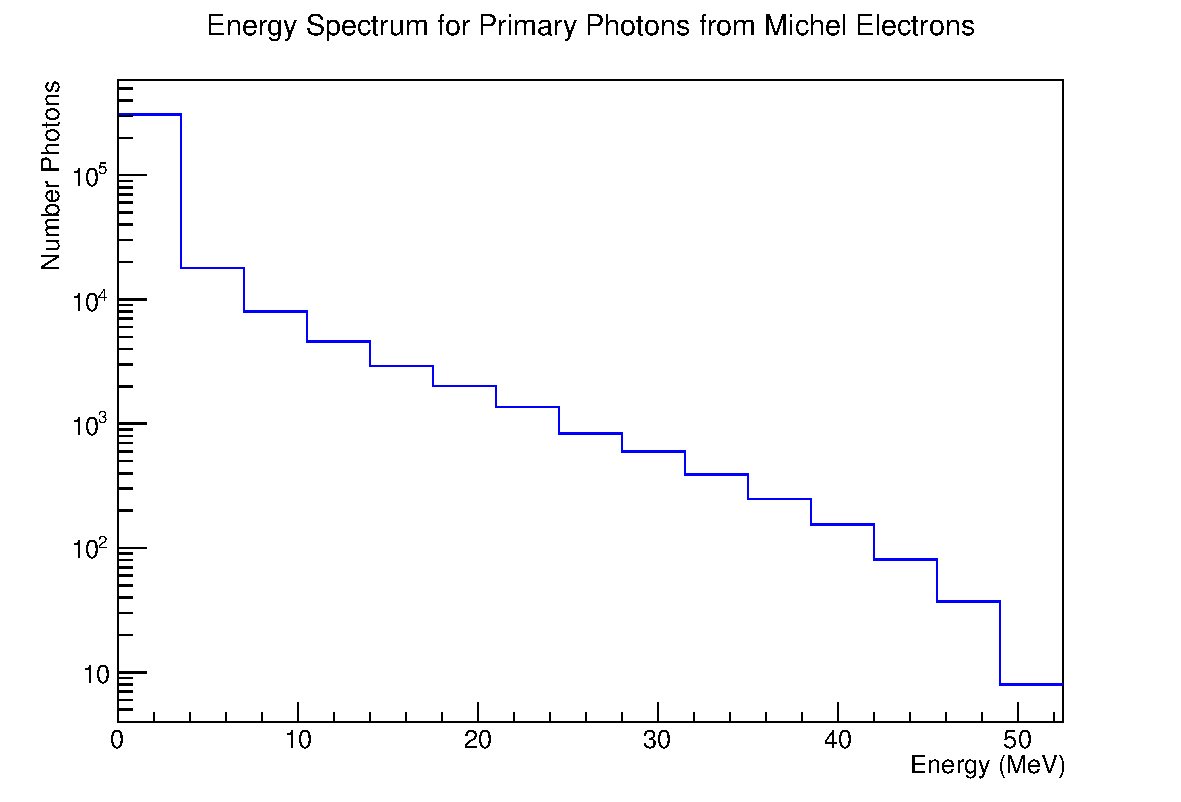
\includegraphics[width=\textwidth]{figures/photon_spec.pdf}
		\caption[Photon energy spectrum.]{Photon energy spectrum.}
		\label{fig:photon_spec}
	\end{subfigure}

	\vspace{5mm}

	\begin{subfigure}[b]{\textwidth}
		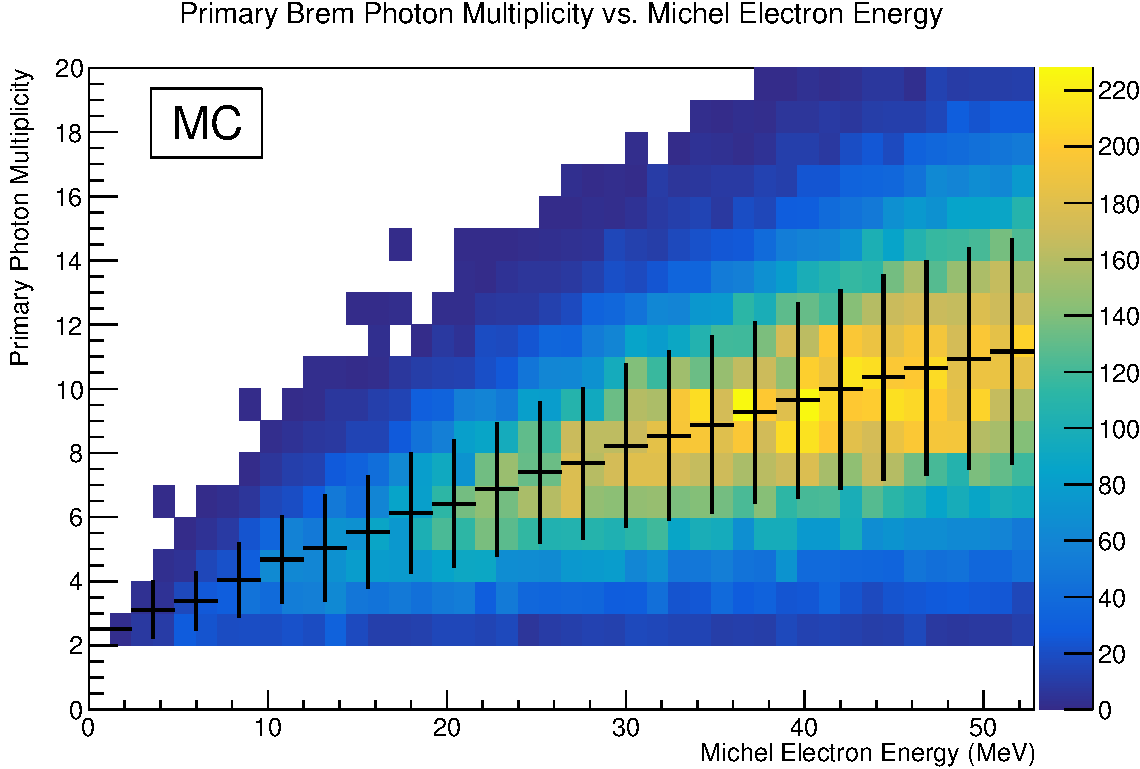
\includegraphics[width=\textwidth]{figures/photon_mult.pdf}
		\caption[Photon multiplicity.]{Photon multiplicity as a function of true
		Michel electron energy.}
		\label{fig:photon_mult}
	\end{subfigure}

	\caption
	[Properties of radiated energy deposits from Michel electrons.]
	{Properties of radiated energy deposits from Michel electrons in \protodune{}
	simulation.} 

	\label{fig:photon_prop}

\end{figure}

The energy which is lost into radiated photons is only visible once the photons
interact in the argon to produce secondary electrons which then ionise the
argon. These secondary electrons are scattered over large angles and distances
in the detector when compared to the short Michel electron track, the spatial 
distribution of secondary electrons is shown in Figure \ref{fig:photon_geom}.
This shows that the radiated energy deposits are spread over a large area, when
compared to the size of the initial Michel electron track. Therefore, any 
reconstruction algorithm hoping to recover the radiated energy, will 
need to use data from a relatively large volume in order to maximise energy
recovery.
\begin{figure}
	\centering
	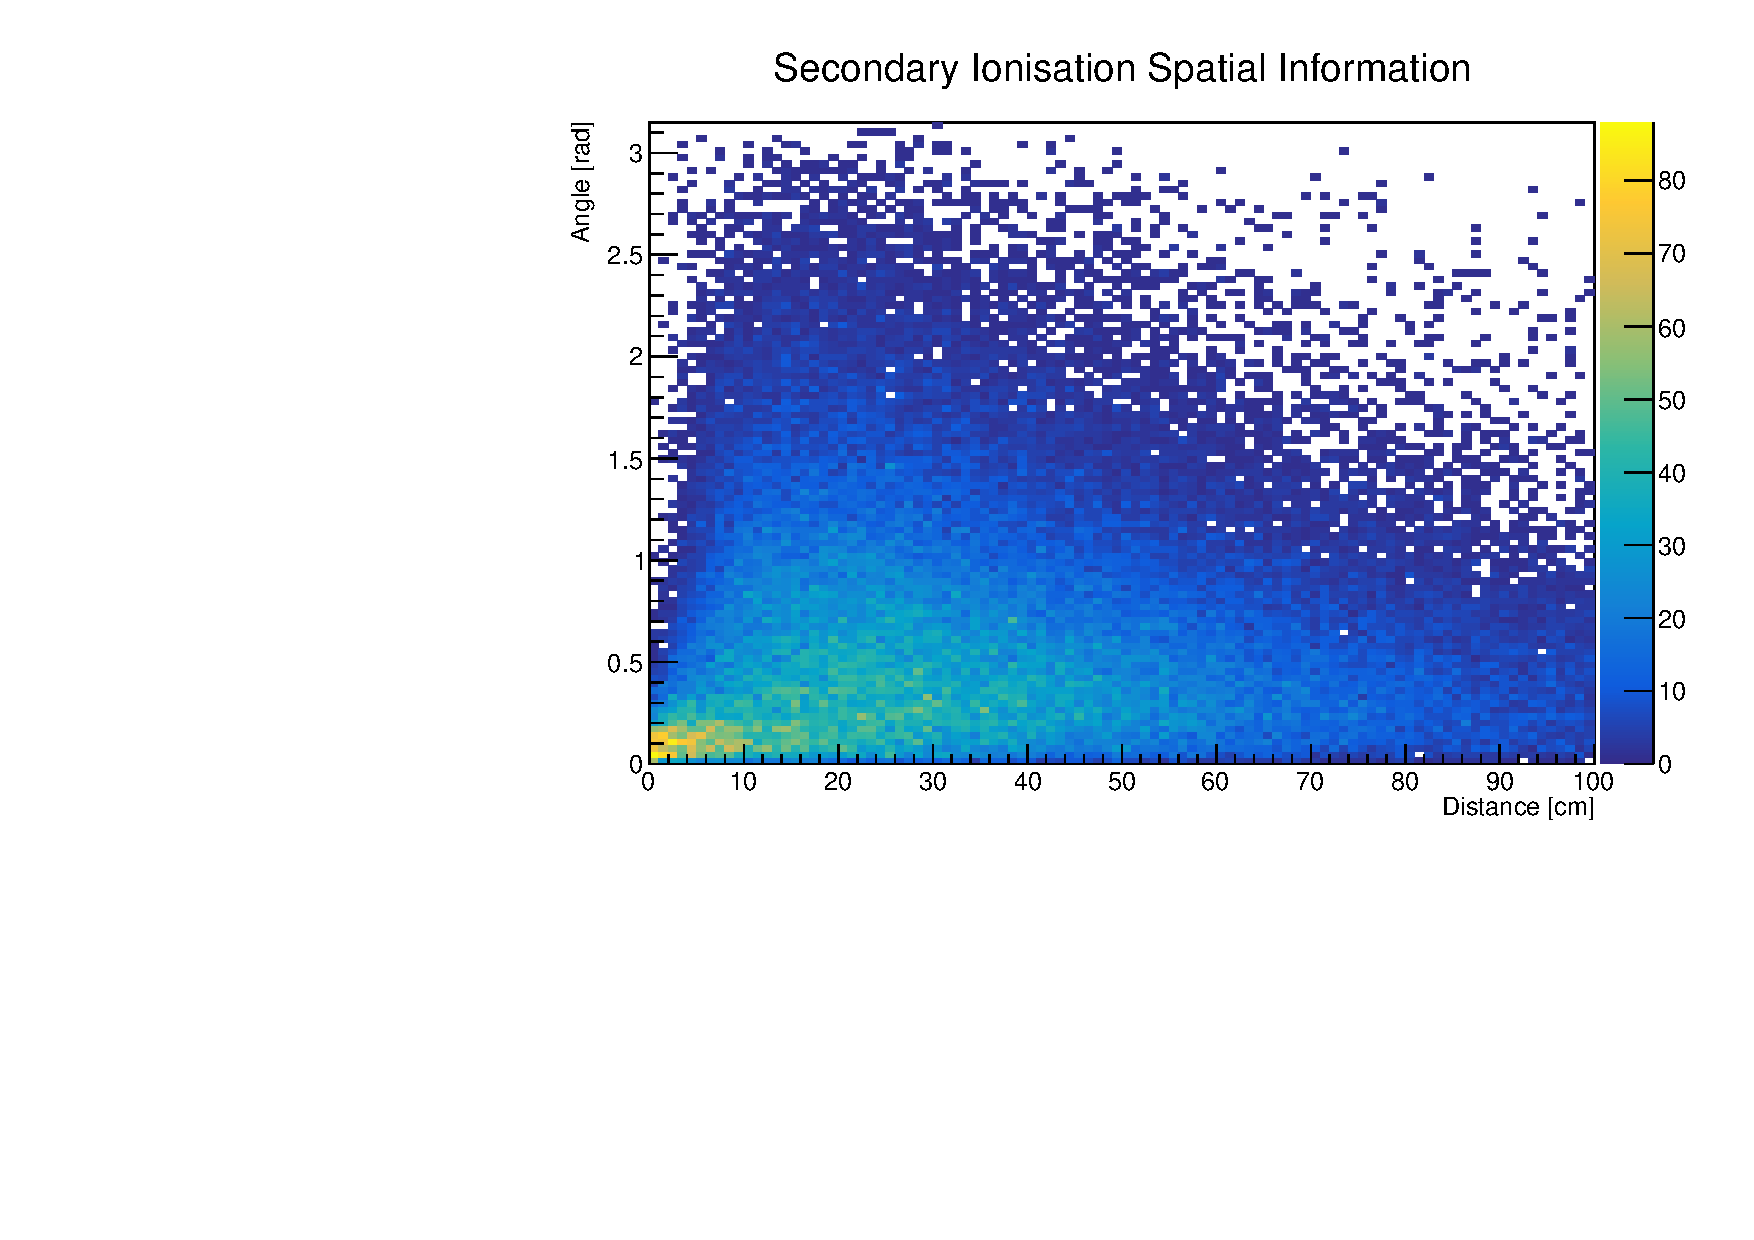
\includegraphics[width=\textwidth]{figures/photon_geom.pdf}
	\caption
	[Spatial distribution of radiated ionisation deposits.]
	{Spatial distribution of radiated ionisation deposits.}
	\label{fig:photon_geom}
\end{figure}

To highlight the impact of the radiated energy deposits we can consider the 
results of perfect energy reconstruction in two cases:
\begin{itemize}
	\item Only considering the Michel electron track.
	\item Considering all ionisation energy within some radius and angle of the 
		Michel electron track.
\end{itemize}
Figure \ref{fig:michel_track_only} illustrates the considerable increase in energy
collected if radiated energy is considered. The distribution is significantly
narrower and much more energy is recovered when considering the energy deposited
within a sphere of height $40\mbox{ cm}$ and angle 30\textdegree of the Michel 
electron vertex. In addition, the fraction of energy recovered as a function of
Michel electron energy has a more linear distribution for a collection radius of
40 cm.
\begin{figure}
	\centering

	\begin{subfigure}[b]{\textwidth}
		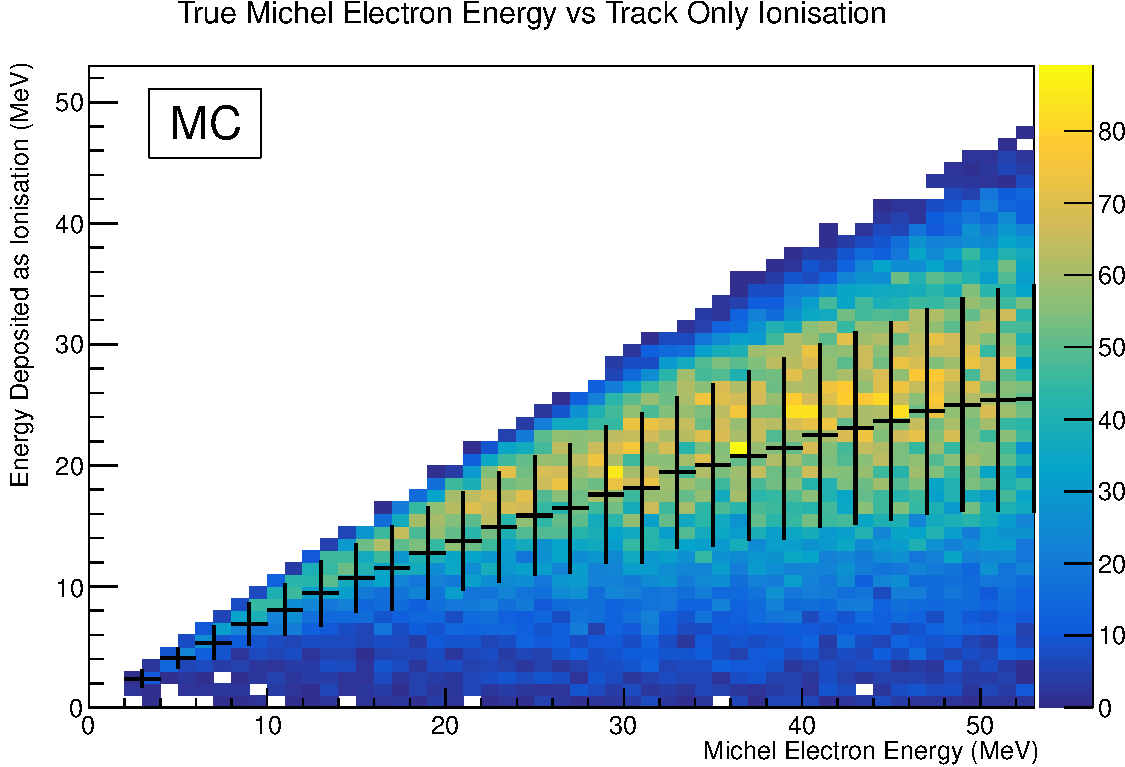
\includegraphics[clip, trim = 0cm 0cm 0cm 1cm, width=\textwidth]{figures/michel_track_only.pdf}
		\caption
		[Initial Michel electron track only.]
		{Initial Michel electron track only.}
		\label{fig:track_only}
	\end{subfigure}

	\vspace{5mm}

	\begin{subfigure}[b]{\textwidth}
		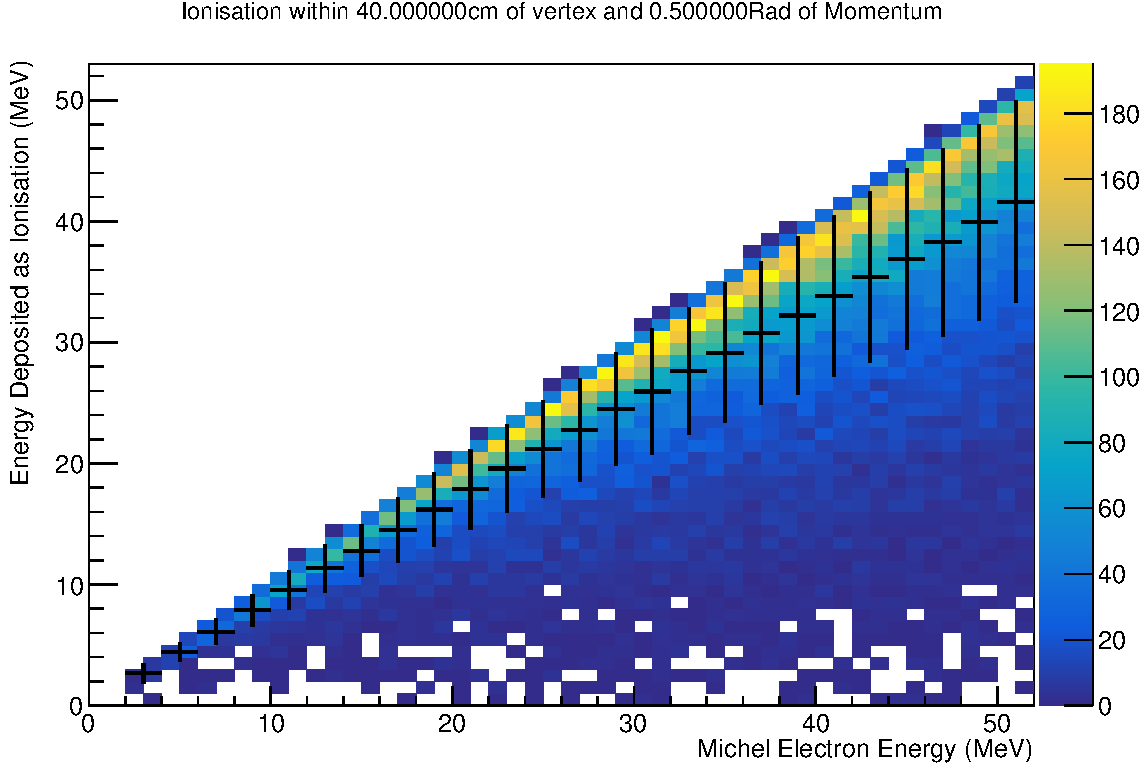
\includegraphics[clip, trim = 0cm 0cm 0cm 1cm, width=\textwidth]{figures/cone_reco.pdf}
		\caption
		[Ionisation withing a 40 cm cone at $30^\circ$ opening angle.]
		{Ionisation withing a 40 cm cone at $30^\circ$ opening angle.}
		\label{fig:cone_reco}
	\end{subfigure}

	\caption
	[Available ionisation energy vs true Michel electron energy.]
	{Available ionisation energy vs true Michel electron energy.}

	\label{fig:michel_track_only}

\end{figure}

The average fractional energy recovery as a function of collection radius is
shown in Figure \ref{fig:frac_v_radius}, where the error bars represent the RMS
of the distribution. By increasing the collection radius from 0 cm to 40cm, 
the average energy recovered is increased from 57\% to 87\%. The RMS of the
fractional energy recovered reduces slightly from 20\% to 16\% across this
range. Therefore, the spread in the fraction of energy recovered is reduced 
from 35\% to 18\%. 
\begin{figure}
	\centering
	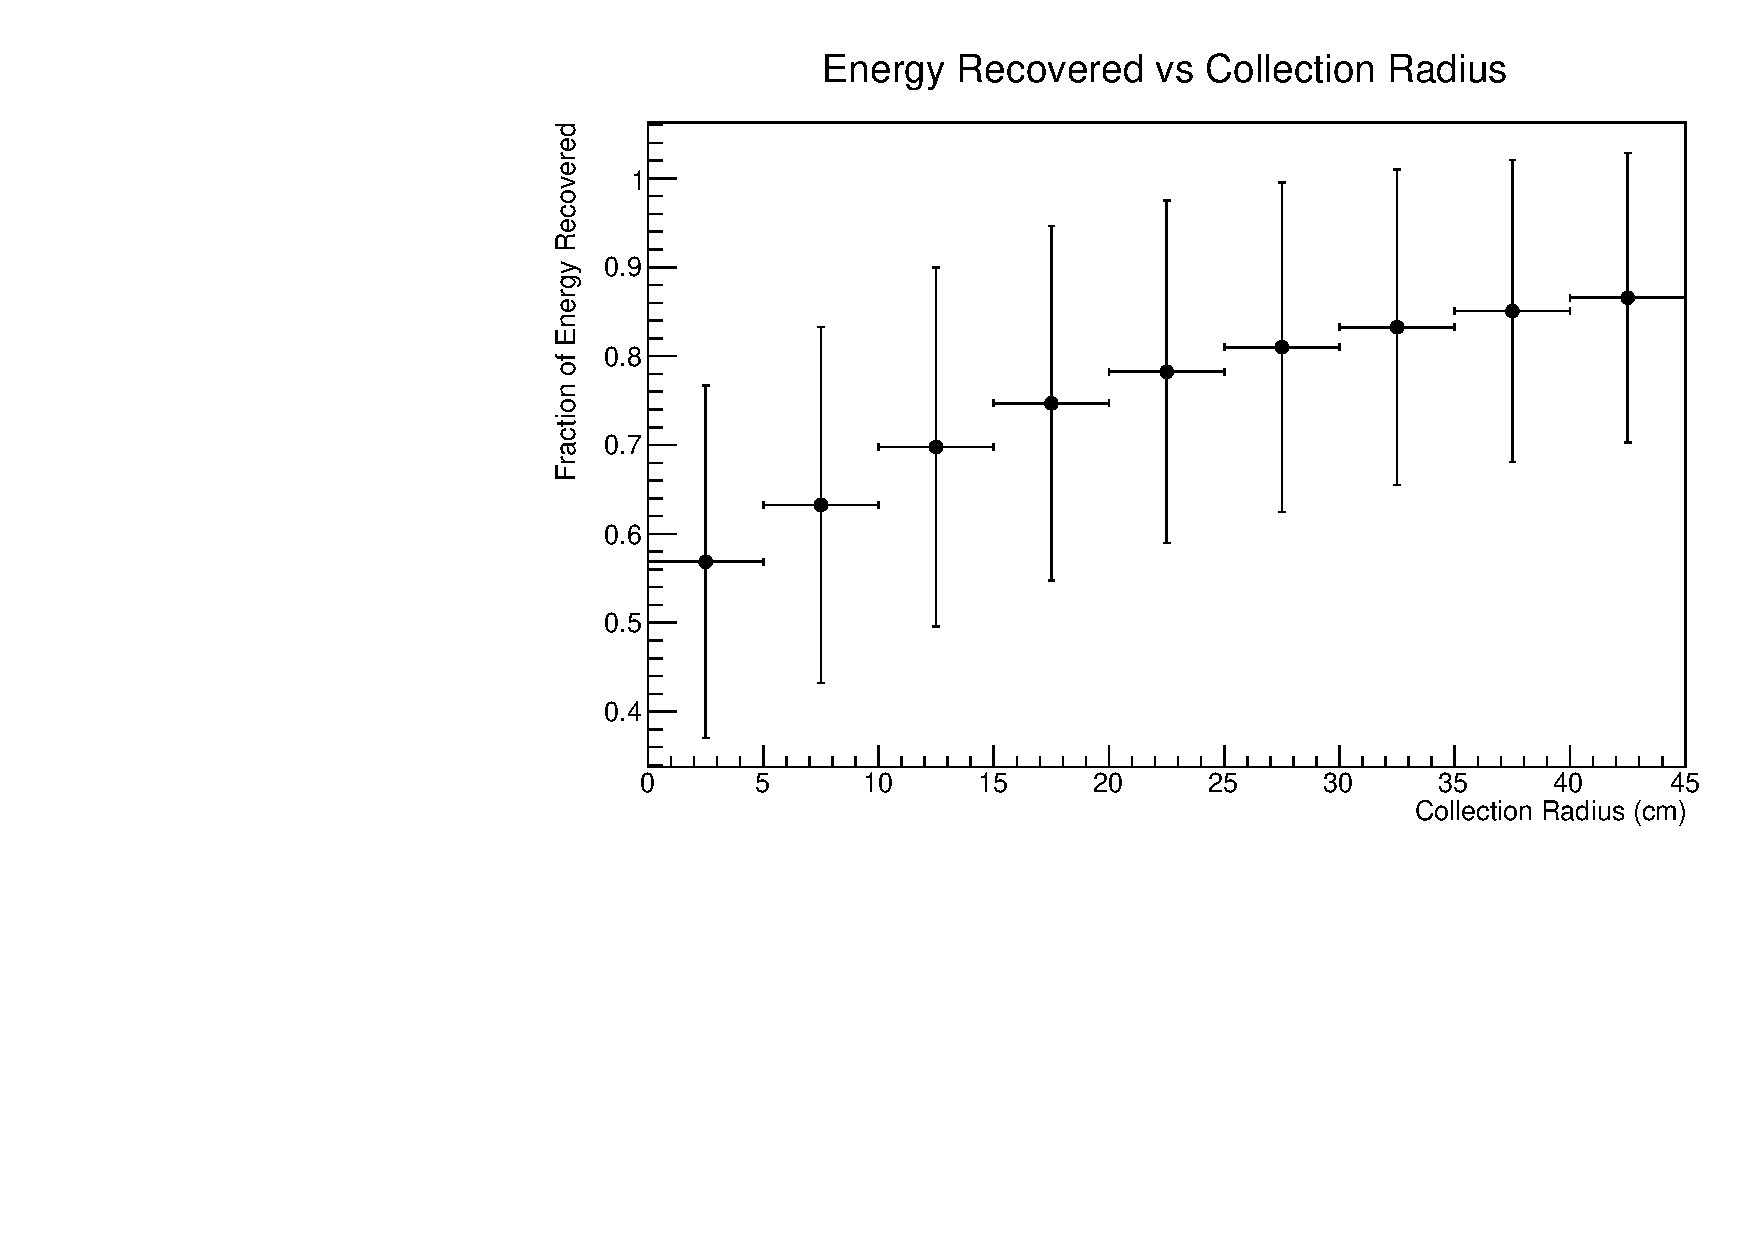
\includegraphics[width=\textwidth]{figures/energy_recovery_v_radius.pdf}
	\caption
	[Fraction of Michel electron energy collected vs collection radius.]
	{Fraction of Michel electron energy collected vs collection radius.}
	\label{fig:frac_v_radius}
\end{figure}

Increasing the collection radius beyond around 30--40 cm gives minimal
improvement in the fractional energy recovery from ionisation. However, it is
likely to impact the purity and efficiency of reconstruction algorithms.
Therefore, the energy reconstruction algorithm discussed in this chapter
considers a 40 cm collection radius when collecting radiated energy deposits.

The MC study presented here highlights the importance of radiated energy
deposits in Michel electron and other low--energy electron events. Based on
these results it is clear that to minimise energy uncertainties for these events
it is important to maximise the amount of energy collected from radiated 
photons. The rest of this chapter will discuss an algorithm which was developed 
to tackle this problem, and it's application on Michel electron events in 
\protodune{} data.

\section{Michel Electron Event Selection} \label{ME_ES}
In order to select Michel electrons in \protodune{} data, an event selection
algorithm was developed based on combining the results from the hit tagging CNN 
from the previous chapter with clustering performed by the main \protodune{} 
reconstruction framework, Pandora. 

The event selection algorithm has four steps:
\begin{enumerate}
	\item Start with all primary tracks from Pandora.
	\item Define a set of Michel electron candidates from the list of all
		daughters of the track.
	\item Find the best Michel electron candidate from the list of Michel electron
		candidates.
	\item Select events where the best Michel electron candidate passes the event
		selection cuts.
\end{enumerate}

First, the initial sample of muon candidates is defined. All tracks from the 
Pandora reconstruction chain which have been labelled as primary tracks are 
considered.

The second step defines a set of Michel electron candidates for each muon
candidate. A Michel electron candidate is any daughter of the primary Pandora
track which satisfies the following conditions:
\begin{itemize}
	\item Starts within 5 cm of the primary track endpoint.
	\item Contains a minimum of 5 reconstructed hits on the collection plane.
\end{itemize}

In the third step, the Michel electron candidates are analysed in order to 
define the best Michel electron candidate for each muon candidate. The best 
Michel electron candidate is the Michel electron candidate with the largest 
fraction of Michel--like hits based on the output of the Michel electron score 
from the CNN. A threshold of 0.9 is used to identify hits as Michel--like. In 
the case of a tie the Michel electron candidate with the most hits is chosen.

The fourth step is the final decision, which is based on the fraction of Michel
like hits in the best Michel electron candidate. Events are selected if the 
best Michel electron candidate is made up of more than 80 \% of Michel--like 
hits. Figure \ref{fig:michel_like_frac} shows a comparison of the fraction of 
Michel--like hits in Michel electron candidates for \protodune{} data and 
simulation. There is a good agreement between data and simulation. The pile--up
of events at one corresponds to Michel electron candidates where all hits were 
classified as Michel--like.
\begin{figure}
	\centering
	% TODO: Remake this plot
	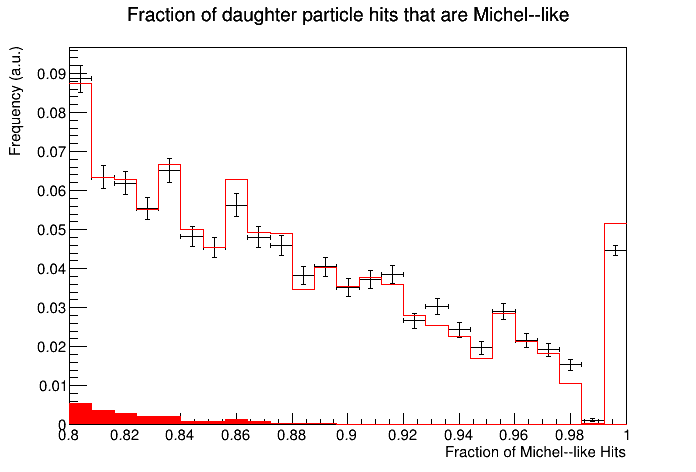
\includegraphics[width=\textwidth]{figures/michel_like_frac.png}
	\caption
	[Fraction of Michel--like hits in the best Michel electron candidate.]
	{Fraction of Michel--like hits in the best Michel electron candidate.}
	\label{fig:michel_like_frac}
\end{figure}

Based on this algorithm Michel electron events are selected with an average
purity of \mccorrect{TODO \%} and an average efficiency of \mccorrect{TODO \%} 
in \protodune{} simulation. Figure \ref{fig:eff_and_pur} shows the
distribution of event selection efficiency and purity as a function on Michel
electron energy. \mccorrect{TODO, analysis and figure.}
\begin{figure}
	\centering
	% TODO: Remake these plots.
	\begin{subfigure}[b]{\textwidth}
		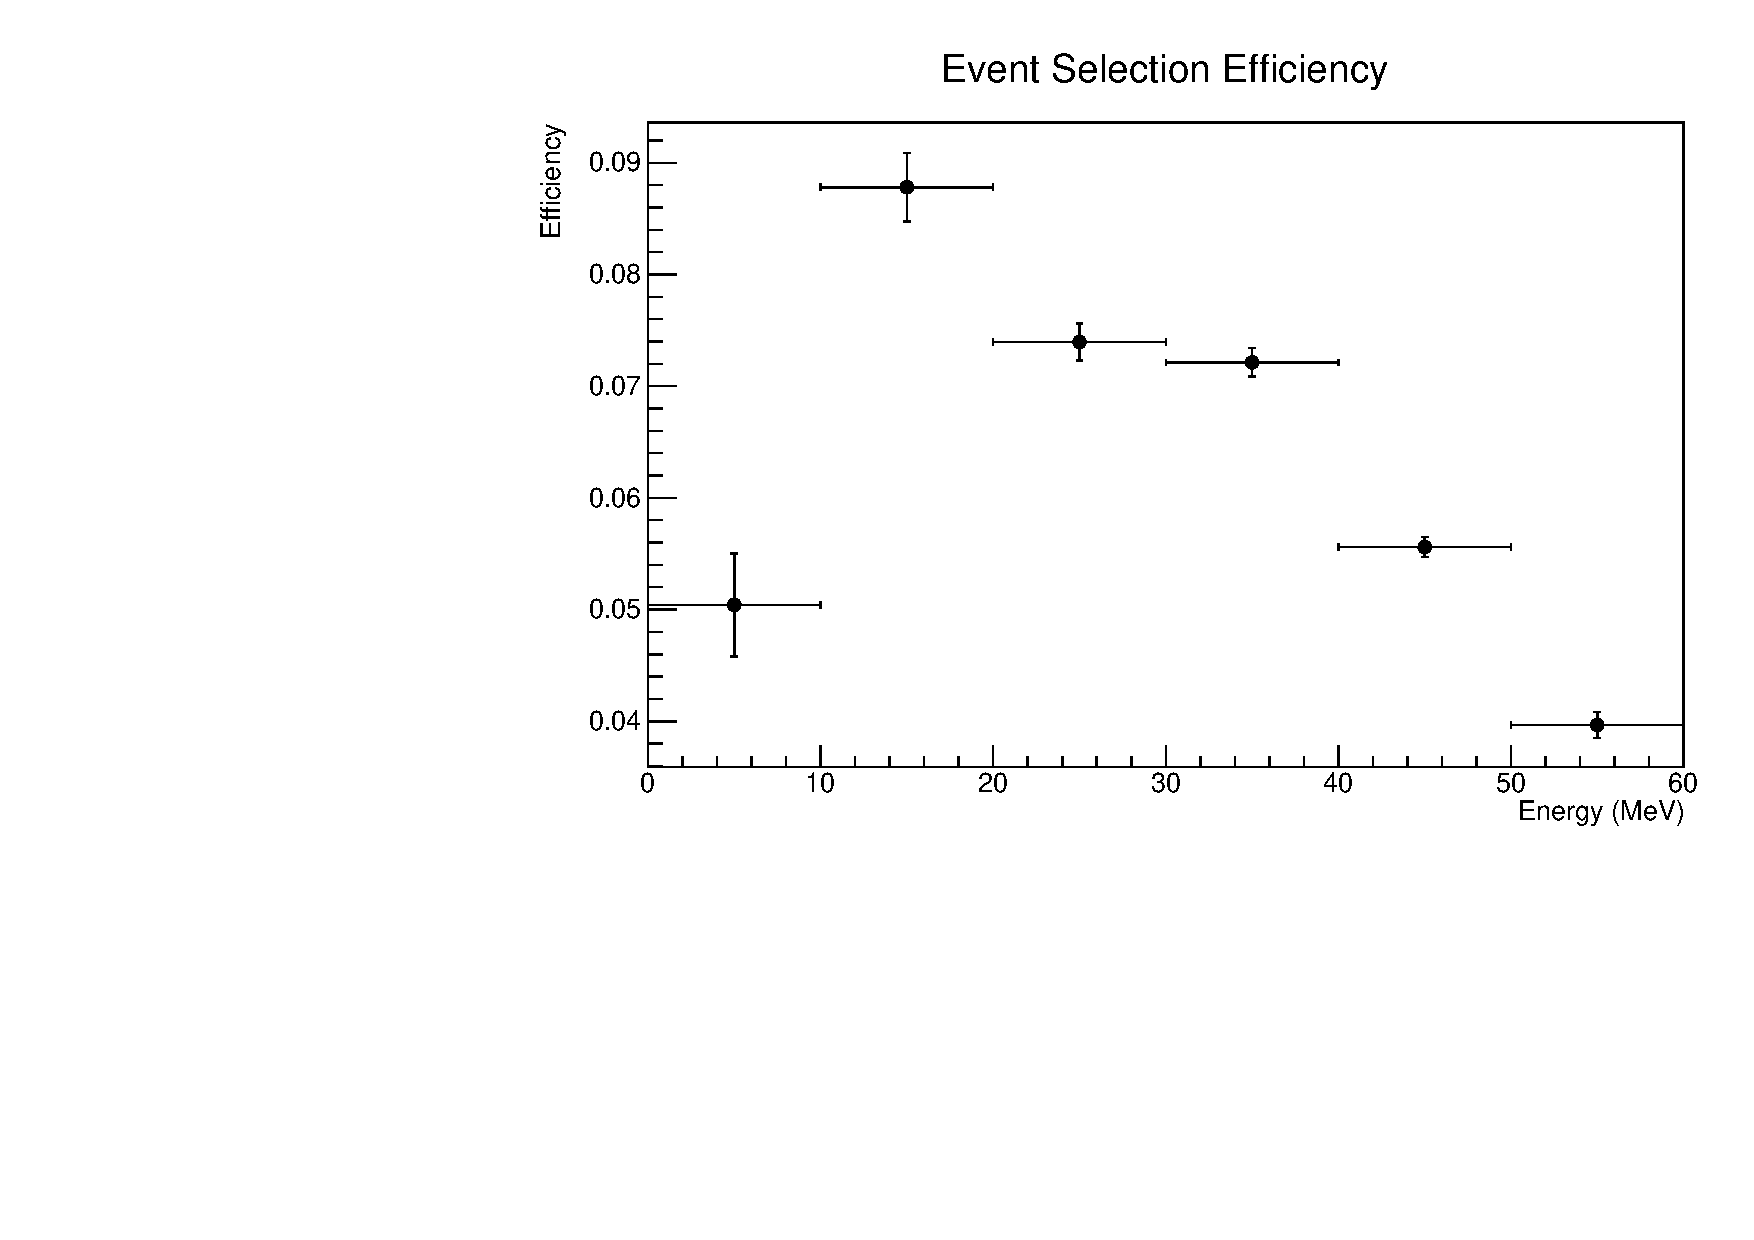
\includegraphics[width=\textwidth, height=0.68\textwidth]{figures/eff_v_energy.pdf}
		\caption
		[Purity vs True Michel electron energy.]
		{Purity vs True Michel electron energy.}
		\label{fig:eff_v_energy}
	\end{subfigure}
	\begin{subfigure}[b]{\textwidth}
		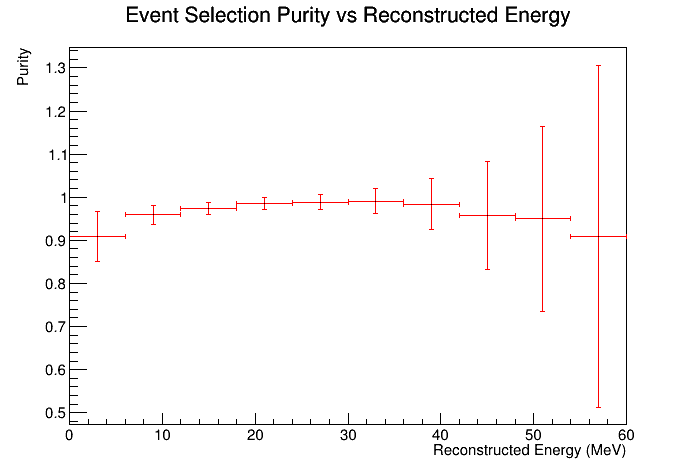
\includegraphics[width=\textwidth]{figures/MC_purity_v_energy.png}
		\caption
		[Efficiency vs True Michel electron energy.]
		{Efficiency vs True Michel electron energy.}
		\label{fig:pur_v_energy}
	\end{subfigure}

	\caption
	[Purity and efficiency of Michel electron event selection as a function of
	energy.]
	{Purity and efficiency of Michel electron event selection as a function of
	energy.}

	\label{fig:eff_and_pur}

\end{figure}

\mccorrect{TODO, muon kinematic distributions.}

\section{Michel Electron Energy Reconstruction} \label{ME_R} 
% \begin{mccorrection}
% 	\begin{itemize} 
% 	\item U-Nets and semantic segmentation
% 	\item Algorithm outline
% 	\item Details of my U-Net
% 	\item Architecture plot
% 	\item Map examples
% 	\item Data v MC score distribution
% 	\item Reco spectrum
% 	\item NHits
% 	\item Energy per hit
% 	\item Reco geometry variables
% 	\end{itemize}
% \end{mccorrection}

To reconstruct the energy of Michel electrons in liquid argon the relevant hits
must first be selected. Once the hits are selected the ionisation energy
deposited by each hit is then reconstructed, the reconstructed energy of the 
Michel electron is the sum of the reconstructed energy of all relevant hits. In
this section we will detail a hit selection algorithm based on a type of
convolutional neural network called a U-Net, which returns hit selection maps 
for the Michel electron energy reconstruction. This algorithm is used to select 
Michel electron hits with a high purity and efficiency, the resulting 
reconstructed energy spectrum is used to estimate the energy resolution of 
\protodune{} for electrons in the tens of MeV range.

\subsection{Michel Electron Hit Tagging with U-Nets}

A U-Net is a type of convolutional neural network which is designed to perform
semantic segmentation of images \cite{TODO}. In semantic segmentation the goal
of the network is to return a map of pixels which correspond to the areas of 
interest; the output of the network is the same dimension as the input with a 
one--to--one correspondence between input pixels and output pixels. The
architecture used for the hit selection algorithm is shown in Figure
\ref{fig:unet_arch}. During the first half of the network architecture the
resolution of the output is decreases, this is analogous to many conventional
CNN's and during this phase the network learns about the content of the image.
The second phase of the architecture allows the U-Net to rebuild the locations 
of different features within the initial image, this is achieved by passing 
the details of previous layers to the network as the resolution of the output 
map is slowly increased back to the original resolution \cite{TODO}. 

\mccorrect{TODO: improve the architecture description.}

In the Michel electron case, the goal of the network is to return a map of all
ionisation energy deposits which come from the Michel electron, this includes
the initial track and any secondary deposits from radiated photons. The inputs
and outputs are two dimensional images of the location of reconstructed hits
centered on the selected Michel electron. The amplitude of each input pixel is 
given by the integrated charge of any reconstructed hits within the pixel. For
the outputs the pixels have an amplitude of 1 if they contain a Michel electron
hit, and 0 otherwise. Only data from the collection plane is used because there 
is a higher signal to noise ratio on these wires. 

Intersection--over--union was used as the loss function for the U-Net. This loss
is defined as 
\begin{equation}
	\mbox{IOU}(A, B) = \frac{|A \cap B|}{|A \cup B|}
\end{equation}
where $A$ is the set of all selected hits, and $B$ is the set of all true hits.
This loss rewards the network for selecting as many correct hits as possible
(high intersection), while penalising it for selecting more hits than it needs
to (high union). The IOU score lies between 0 and 1, with a score of 1
corresponding to a perfect match between the two sets and therefore perfect hit
tagging in our Michel electron case.

The network architecture used for the Michel electron reconstruction is shown in
Figure \ref{fig:unet_arch}. The network consists of a repeating structure which
contains the following key components:
\begin{itemize}
	\item Convolutional layers in the form of inception units.
	\item Pooling layers for downscaling.
	\item Residual connections and up--sampling.
\end{itemize}
FIXME. \mccorrect{Description}. As with the hit tagging CNN from the previous chapter, 
both dropout and early--stopping are implemented to prevent over--fitting.
\begin{figure}
	\centering
	% TODO: Make this plot.
	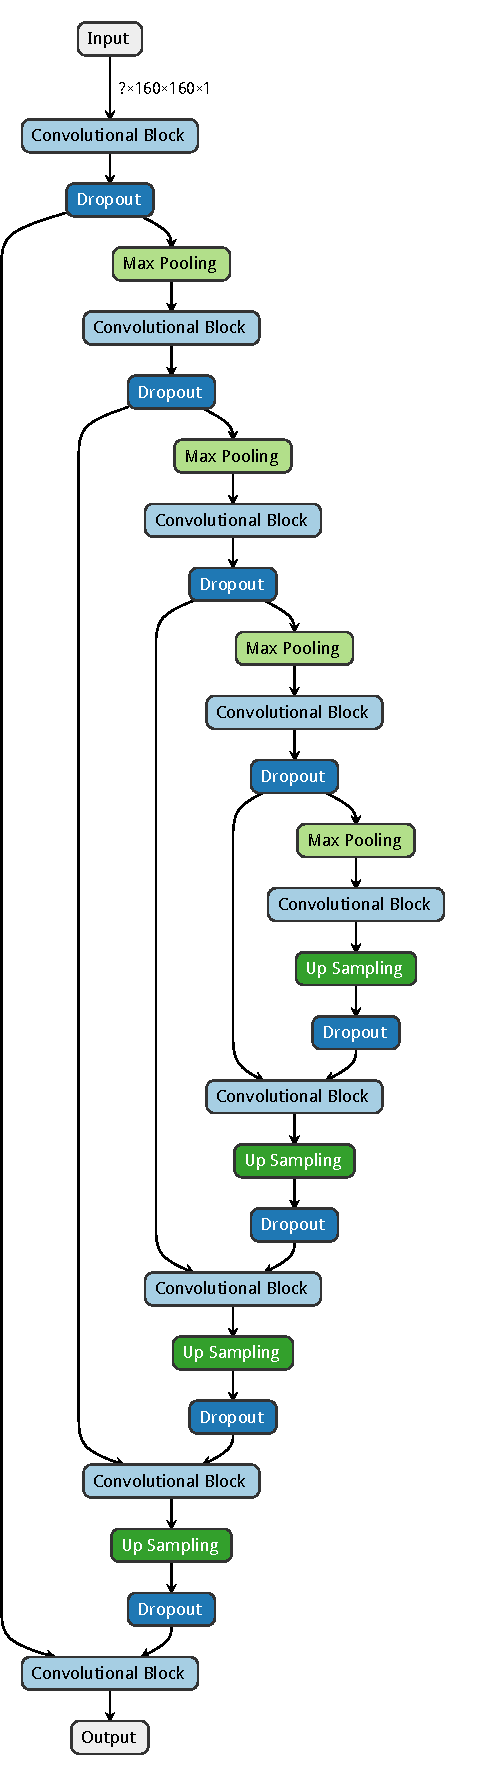
\includegraphics[width=\textwidth, height=0.68\textwidth]{figures/unet_arch.png}
	\caption
	[CNN architecture used to select ionisation energy deposits.]
	{CNN architecture used to select ionisation energy deposits.}
	\label{fig:unet_arch}
\end{figure}

The datasets for the training process were generated from a full simulation of 
the \protodune{} detector under beam operation including both cosmic ray and
beam particles. The images produced contain the location and integrated charge
for each hit within the image window. The training data is split into training, 
test, and validation sets in the ratio 80:10:10. In total around 40,000,000 
images were generated for the training stage.

As with the hit tagging CNN from the previous chapter, the training and
validation scores were monitored throughout training using TensorFlow. The
weights of the network were saved after each epoch, and the final weights were
those from the epoch before the epoch when the validation score first decreased.
Figure \ref{fig:unet_loss} shows the evolution of the loss over time, along with
a vertical line representing the loss at which the weights were chosen.
\begin{figure}
	\centering
	% TODO
	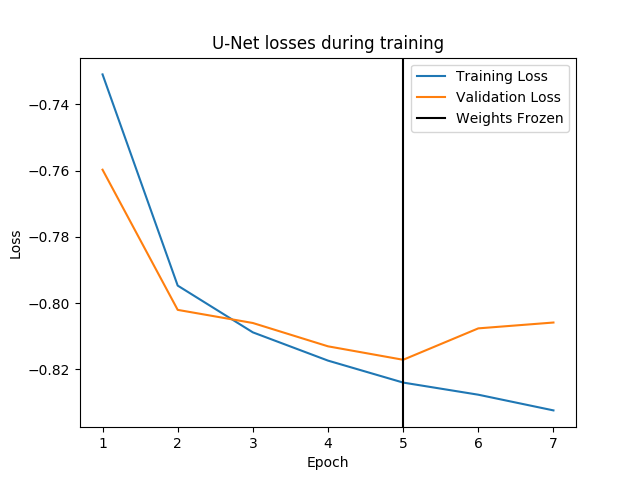
\includegraphics[width=\textwidth]{figures/unet_loss.png}
	\caption
	[U-Net training and validation loss as a function of epoch.]
	{U-Net training and validation loss as a function of epoch.}
	\label{fig:unet_loss}
\end{figure}

A demonstration of the output of the U-Net is given in Figure 
\ref{fig:unet_example} which shows the input, output, and truth images for an 
event from \protodune{} simulation.
\begin{figure}
	\centering
	% TODO
	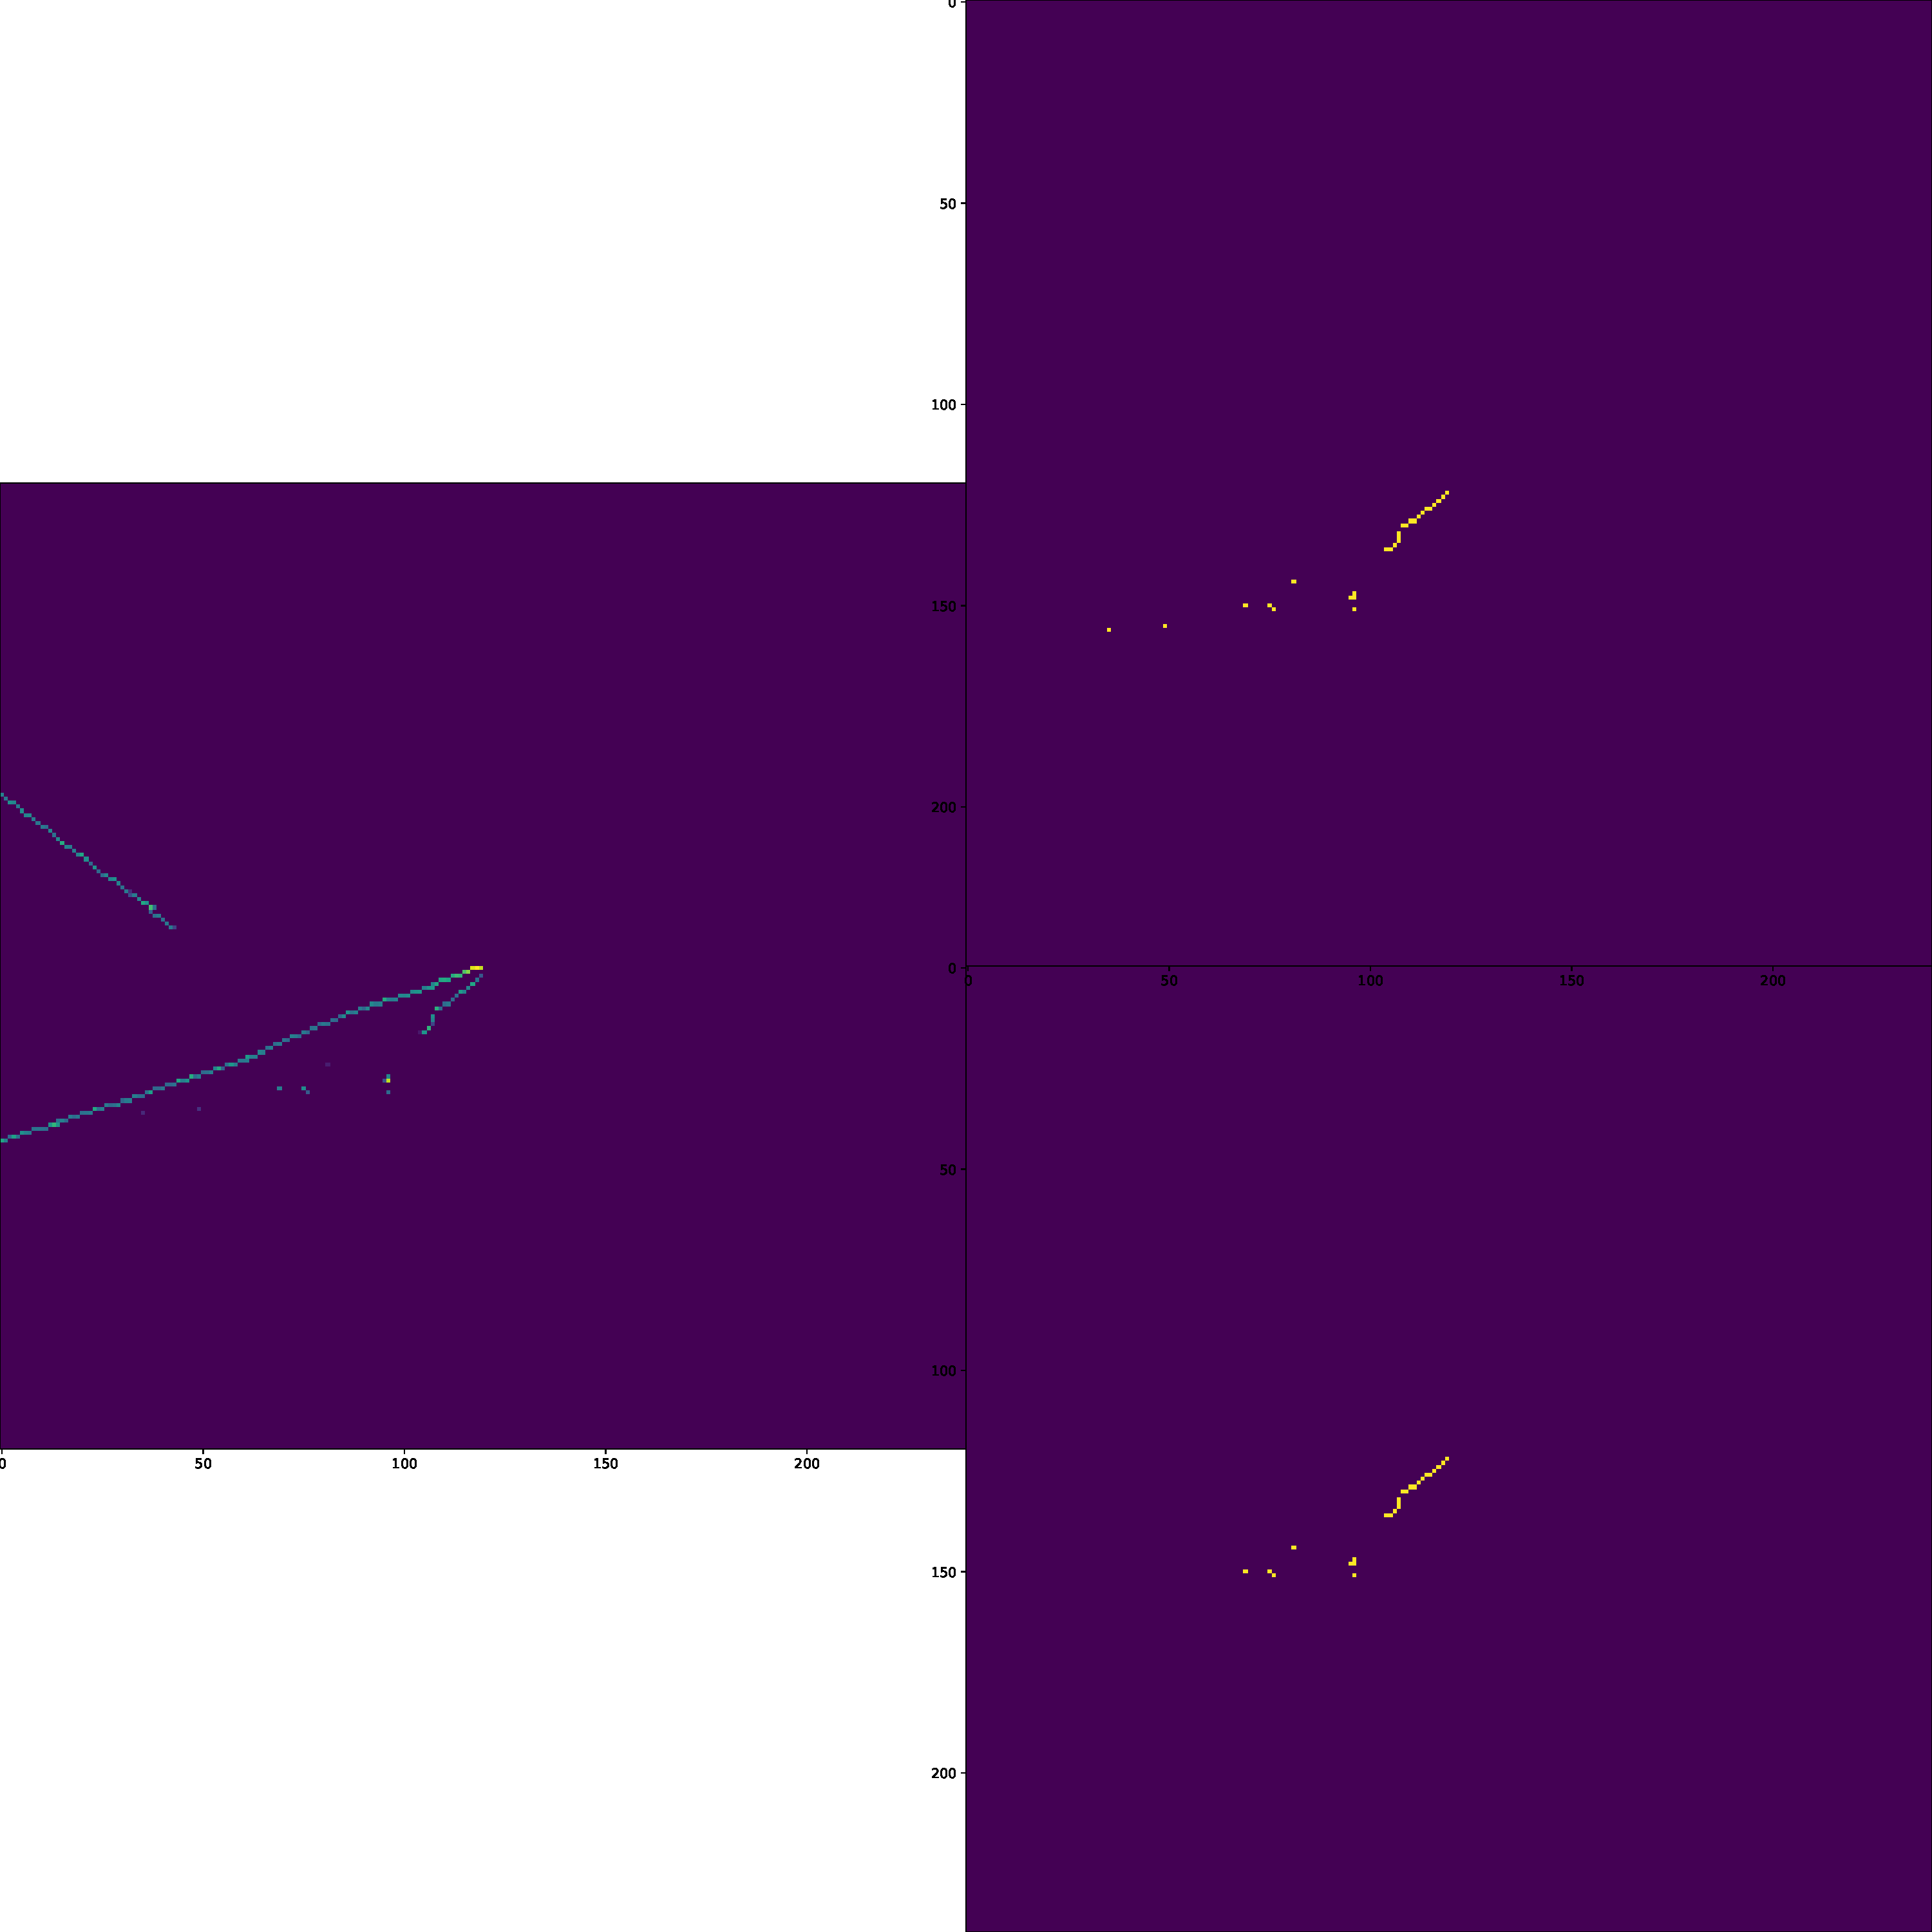
\includegraphics[width=\textwidth]{figures/unet_example.pdf}
	\caption
	[Example input, true output, and prediction images for U-Net.]
	{Example input, true output, and prediction images for U-Net. Left: Input
	image. Top Right: True Output. Bottom Right: U-Net Prediction.}
	\label{fig:unet_example}
\end{figure}

\subsection{Michel Electron Reconstruction}

Michel electron reconstruction was evaluated on a dataset which was part of the 
same batch of simulation as the training, test, and validation data, but
distinct from all of them. 

\subsubsection{Hit Selection}

The U-Net produces a sharply peaked output distribution in both data and
simulation as seen in Figure \ref{fig:unet_pred_data}, which shows sharp peaks
in the distribution at 0 and 1. The distribution has slightly sharper peaks in 
simulation as with seen with the hit tagging CNN from the previous chapter, this
is unsurprising due to the fact that the simulation does not perfectly match the
data. \mccorrect{TODO. Is there a good way to mitigate this?}
\begin{figure}
	\centering
	% TODO
	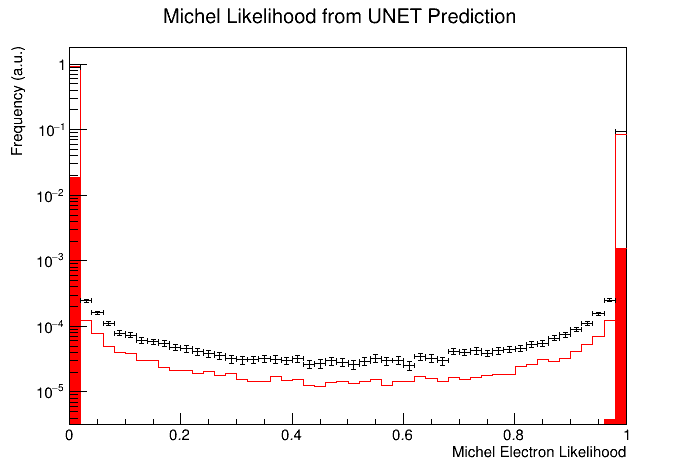
\includegraphics[width=\textwidth]{figures/unet_pred_data.png}
	\caption
	[U-Net Predicted Distribution.]
	{U-Net Predicted Distribution.}
	\label{fig:unet_pred_data}
\end{figure}

Hits from the input images are selected as Michel electron hits if their score
exceed a selection threshold of 0.9. The number of hits selected per event for
data and simulation is shown in figure \ref{fig:mich_n_hits}. Around 10 hits are
selected on average per event, with a slightly larger spread in data than in
simulation.
\begin{figure}
	\centering
	% TODO
	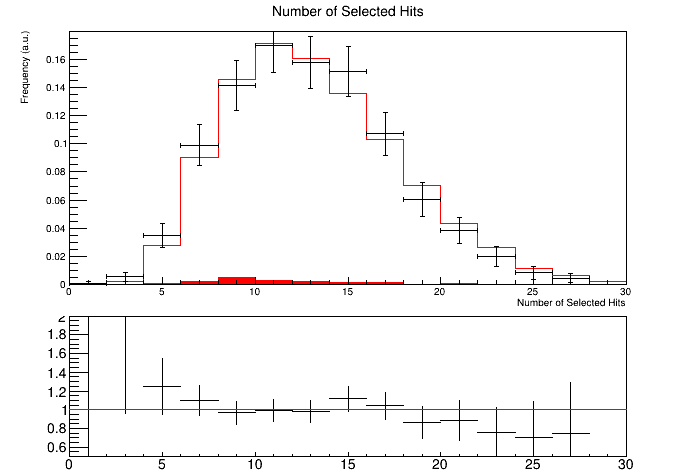
\includegraphics[width=\textwidth]{figures/mich_n_hits.png}
	\caption
	[Number of hits in Michel electron events.]
	{Number of hits in Michel electron events.}
	\label{fig:mich_n_hits}
\end{figure}

The performance of the hit tagging algorithm was analysed with the simulated
sample. The U-Net output distribution for true Michel electron hits and falsely
tagged hits is shown in Figure \ref{fig:unet_pred}, along with a ratio of the
true and false hits as a function of energy. The ratio shows a strong
separation between true hits and false hits, which appear at high scores and low
scores respectively.
\begin{figure}
	\centering
	% TODO
	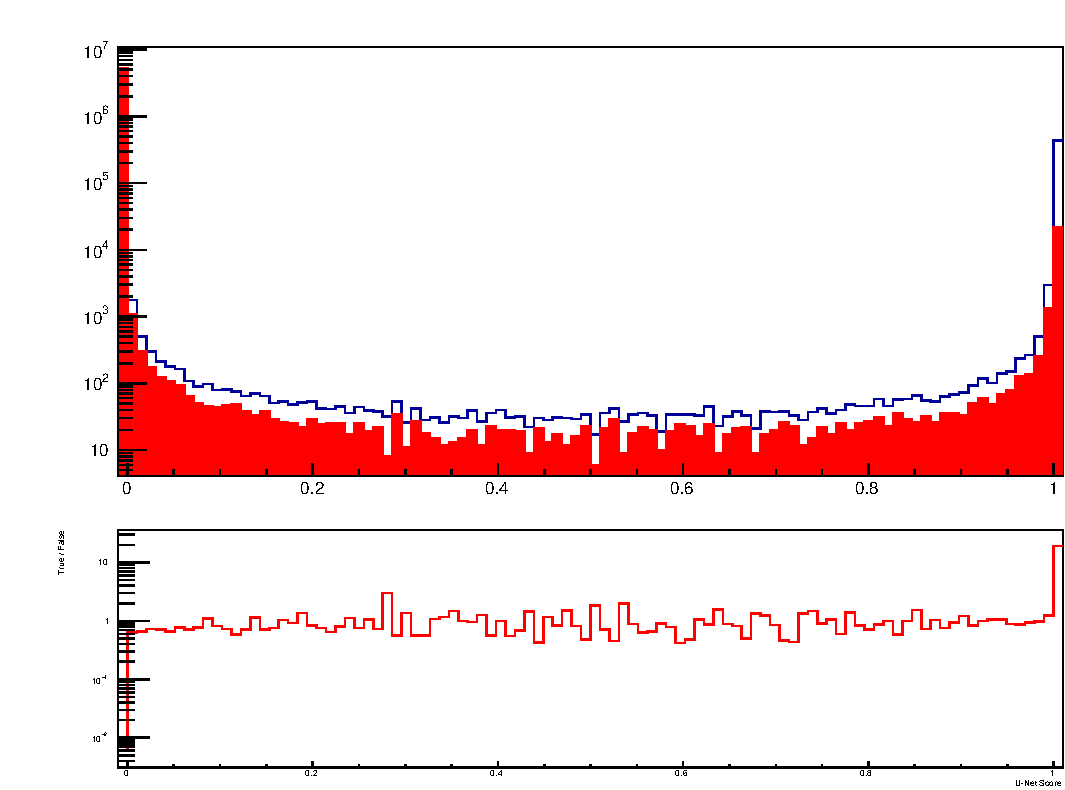
\includegraphics[width=\textwidth]{figures/unet_pred.pdf}
	\caption
	[U-Net output distribution.]
	{U-Net output distribution.}
	\label{fig:unet_pred}
\end{figure}

Based on the score distributions for true and false hits the precision and
completeness of the hit tagging algorithm can be evaluated. The precision and
completeness are defined as 
\begin{align}
	\mbox{Precision} \quad &= \quad  \frac{N_{TP}}{N_{TP} + N_{FP}} \\
	\vspace{2mm}
	\mbox{Completeness} \quad &= \quad \frac{N_{TP}}{N_{TP} + N_{FN}}
\end{align}
where $N_{TP}$, $N_{FP}$, and $N_{FN}$ are the number of true--positive,
false--positive, and false--negative hits respectively. These parameters give a
quantitative evaluation of the performance of the hit tagging algorithm,
allowing for comparison between different algorithms. The purity and
completeness of the hit tagging was calculated for a range of selection
thresholds in the range $[10^{-7}, 1 - 10^{-7}]$, Figure \ref{fig:unet_pur_comp}
shows the purity against completeness for the values in this range. The hit
tagging algorithm produces a high precision and completeness throughout range of
thresholds, however the steepness of the distributions means that the choice of
threshold makes little difference to the performance meaning that little can be
done to optimise the performance by varying the threshold.
\begin{figure}
	\centering
	% TODO
	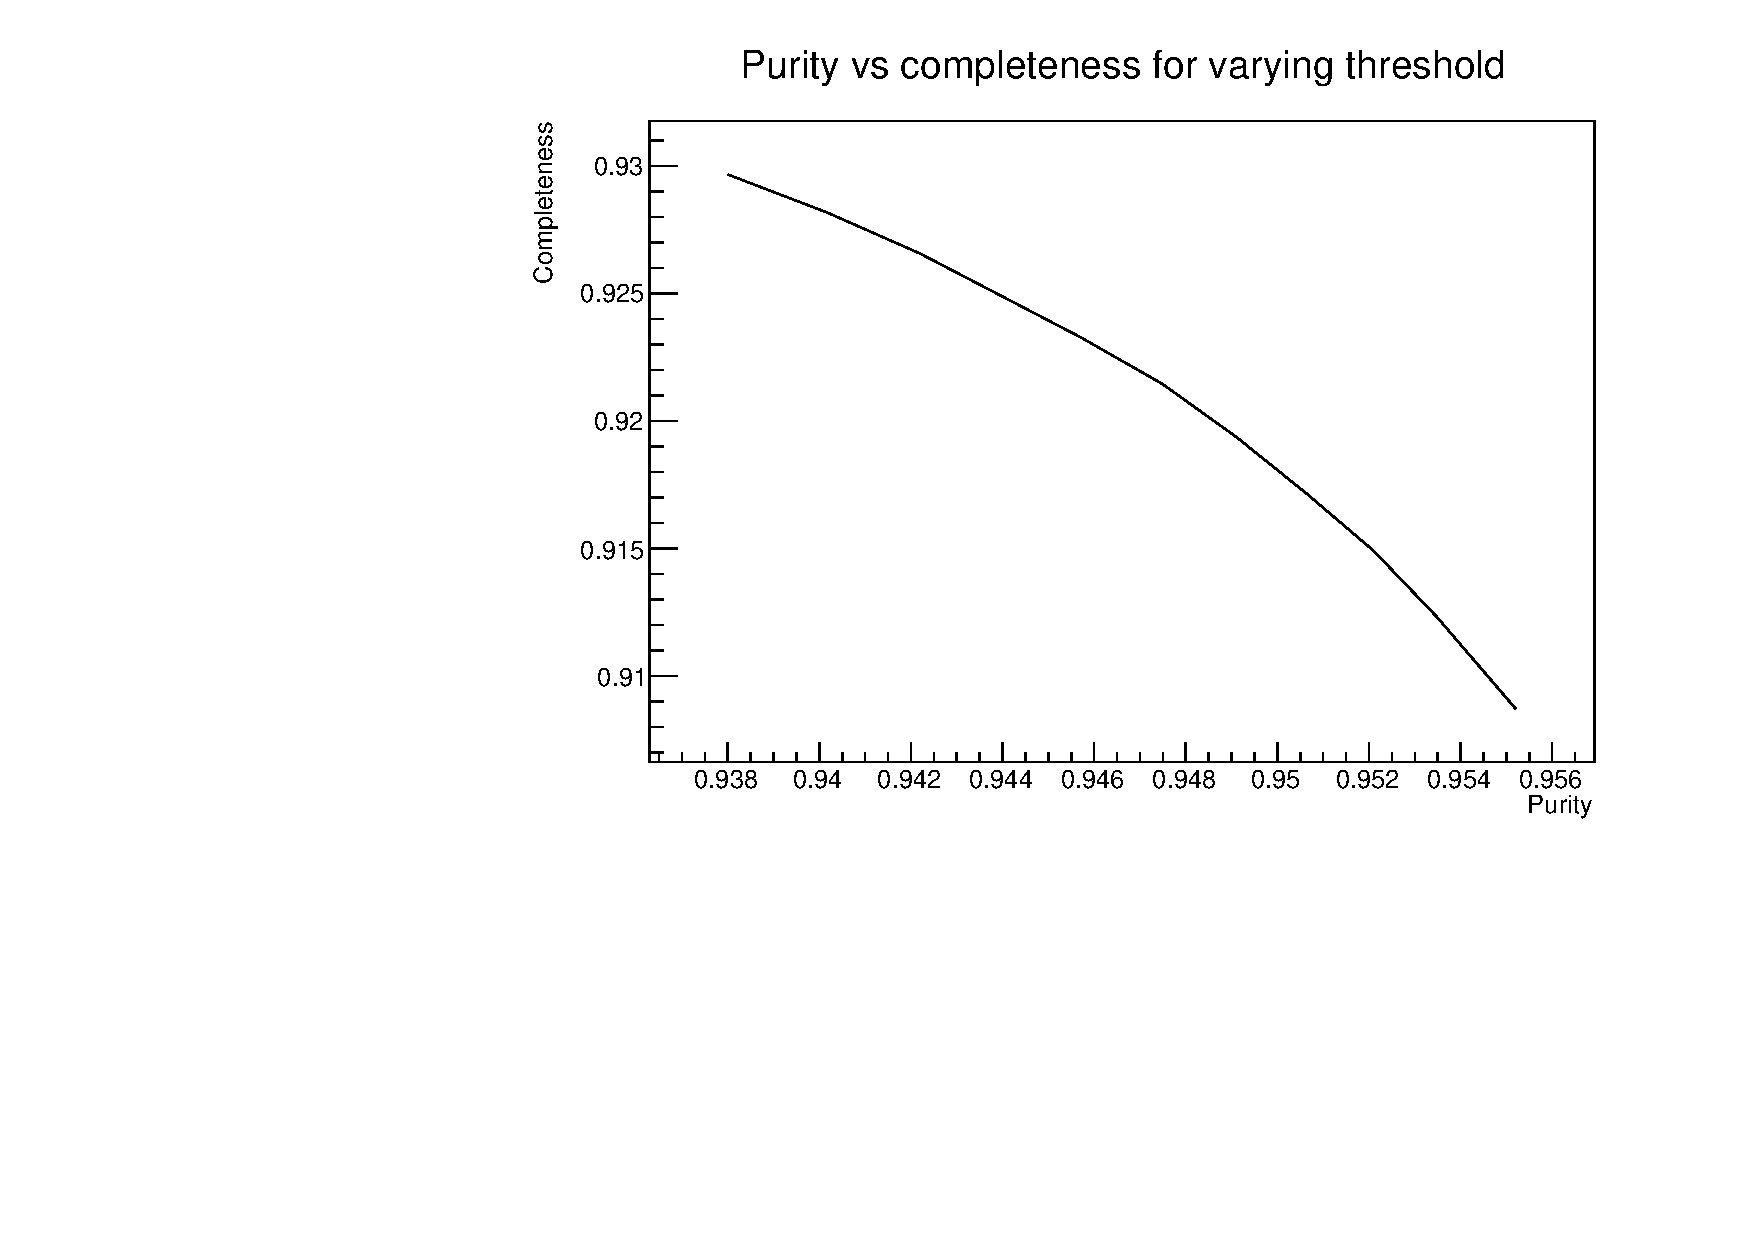
\includegraphics[width=\textwidth]{figures/unet_pur_v_comp.pdf}
	\caption
	[U-Net purity vs completeness.]
	{U-Net purity vs completeness.}
	\label{fig:unet_pur_comp}
\end{figure}

\subsubsection{Ionisation Energy Reconstruction}

The total ionisation energy is reconstructed by summing the hit--by--hit
ionisation energy for all hits selected by the U-Net. The ionisation energy for
each hit is reconstructed from the hit integral in ADC as 
\begin{equation}
	E_{hit} = \frac{I_{hit} \times C_X \times C_{YZ} \times N \times W_{ion}}{C \times R}\mbox{,}
\end{equation}
where $E_{hit}$ is the reconstructed hit energy in MeV, $I_{hit}$ is the
integrated hit charge in ADC, $C_X$ is the X--correction factor which is
dependent on the X coordinate of the hit within the TPC, $C_{YZ}$ is the 
YZ--correction factor which is dependent on the Y and Z coordinates 
of the hit within the TPC, $N$ is a dimensionless normalisation factor which
normalises the data and MC distributions to give the same magnitude, $W_{ion}$
is the ionisation energy of argon in MeV per electron, $C$ is a constant
conversion factor which has units ADC per electron, and $R$ is the
recombination factor. The distribution of reconstructed hit energies in
\protodune{} data and simulation is shown in Figure \ref{fig:hit_ion_reco}.

The position dependent calibration matrices correct for non-uniformity in the
detector response across the TPC. In the X direction the main contributing
factors are attenuation due to electron absorption, and variations in the
electron drift velocity due to space charge effects. The main contributing
factor for the YZ--correction matrix is wire--to--wire response variations.

As discussed in chapter \ref{ch:energyloss} the recombination factor is a
$\frac{dE}{dx}$ dependent factor which depends on the conditions in the liquid
argon. Due to the shortness of Michel electron tracks and the other charge 
deposits it is challenging to assign $\frac{dE}{dx}$ on a hit--by--hit 
basis for this sample, therefore, an average recombination factor is used for 
all hits. The recombination factor is calculated using the box model 
\cite{TODO} under \protodune{} operating conditions to be 0.69.

\begin{figure}
	\centering
	% TODO
	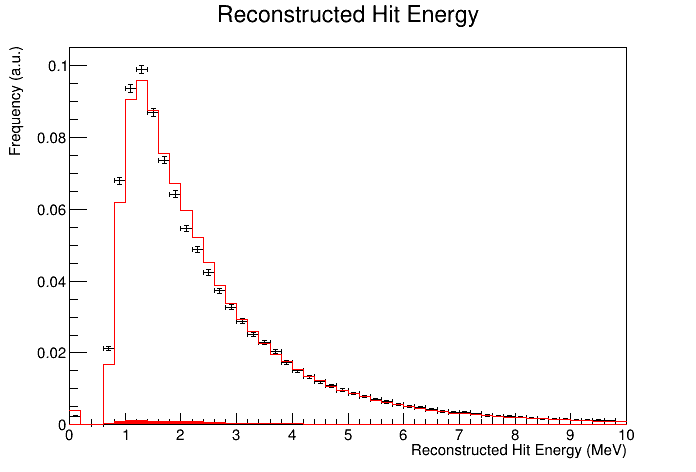
\includegraphics[width=\textwidth]{figures/hit_ion_reco.png}
	\caption
	[Reconstructed Hit Ionisation Energy]
	{Reconstructed Hit Ionisation Energy}
	\label{fig:hit_ion_reco}
\end{figure}

The reconstructed ionisation energy spectrum from Michel electron candidates is
shown in Figure \ref{fig:michel_ion_reco} along with the average ionisation
energy per hit. The distribution peaks at around 18 MeV and has a tail up to 
just under 50 MeV.
\begin{figure}
	\centering
	% TODO
	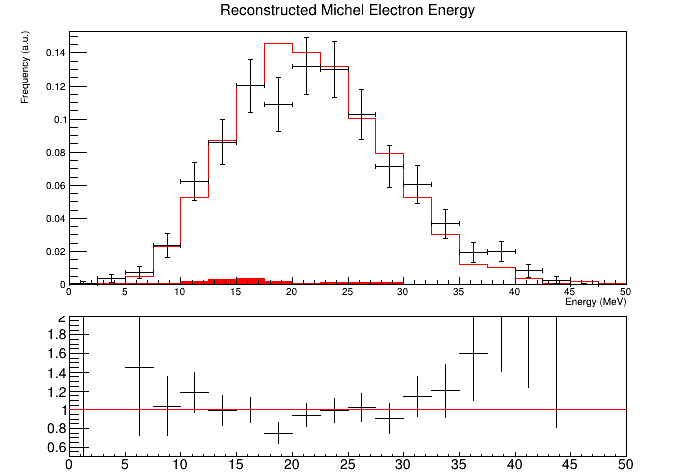
\includegraphics[width=\textwidth]{figures/michel_ion_reco.png}
	\caption
	[Reconstructed Michel Electron Ionisation Energy]
	{Reconstructed Michel Electron Ionisation Energy}
	\label{fig:michel_ion_reco}
\end{figure}

\mccorrect{TODO: analysis of ionisation reconstruction performance.}

\begin{figure}
	\centering
	% TODO: Fix these images
	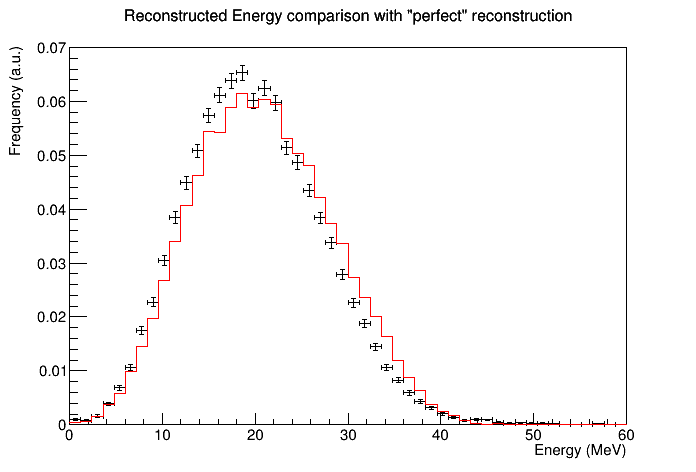
\includegraphics[width=\textwidth, height=0.68\textwidth]{figures/reco_v_ion.png}
	\caption
	[Reconstucted Ionisation vs True Ionisation.]
	{Reconstucted Ionisation vs True Ionisation.}
	\label{fig:reco_v_ion}
\end{figure}

\mccorrect{TODO: Energy resolution fits vs energy.}

\begin{figure}
	\centering
	% TODO: make set of fits as a function of energy
	\includegraphics[width=\textwidth, height=0.68\textwidth]{figures/frac_diff_v_ion.png}
	\caption
	[Fractional energy difference between reconstructed and true Michel electron
	energy.]
	{Fractional energy difference between reconstructed and true Michel electron
	energy.}
	\label{fig:frac_diff_ion}
\end{figure}

\begin{figure}
	\centering
	% TODO: make set of fits as a function of energy
	\includegraphics[width=\textwidth, height=0.68\textwidth]{figures/res_bias_v_ion.png}
	\caption
	[Energy resolution and bias as a function of true ionisation energy.]
	{Energy resolution and bias as a function of true ionisation energy.}
	\label{fig:res_and_bias_ion}
\end{figure}


\subsubsection{Michel Electron Energy Reconstruction}

The true Michel electron energy includes contributions from scintillation light
as well as radiated ionisation energy which is not contained within the images
used in reconstruction. To estimate the total Michel electron energy the
reconstructed ionisation energy needs to be scaled to account for these losses.
As shown in Figure \ref{fig:michel_track_only} there is a none--linear
correlation between the true Michel electron energy and the available ionisation
energy in reconstruction, therefore, a quadratic energy scaling factor was used
to convert the reconstructed ionisation energy into a reconstructed Michel
electron energy. 

The energy scaling factor was estimated by fitting the reconstructed ionisation
energy as a function of true Michel electron energy in \protodune{} simulation
with a quadratic correction as shown in Figure \ref{fig:quadratic_fit}. This 
quadratic is then inverted to give the reconstructed Michel electron energy for 
a given reconstructed ionisation energy, 
\begin{equation}
	E_{michel} = \left( \frac{E_{ion}}{a} - d \right)^{\frac{1}{2}} - \frac{b}{2a},
	\quad d = \frac{c}{a} - \left( \frac{b}{2a} \right)^2 
\end{equation}
where $E_{michel}$ is the reconstructed Michel electron energy, $E_{ion}$ is the
reconstructed ionisation energy, and a, b, and c are the parameters from the
quadratic fit. The fit gives
\begin{equation}
	a = TODO, \quad b = TODO, \quadjc = TODO.
\end{equation}

\begin{figure}
	\centering
	% TODO
	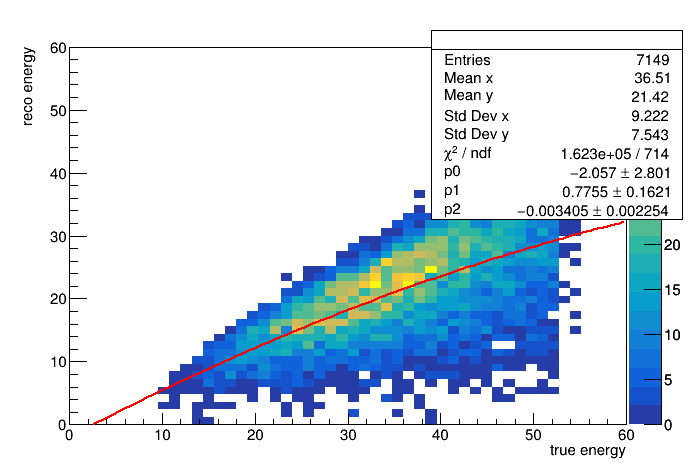
\includegraphics[width=\textwidth]{figures/reco_v_true.png}
	\caption
	[Quadratic Energy Scale Factor.]
	{Quadratic Energy Scale Factor.}
	\label{fig:quadratic_fit}
\end{figure}

The reconstructed Michel electron energy spectrum is shown in Figure
\ref{fig:reco_v_mich}, alongside the true Michel electron energy spectrum from
the simulation. There is a significant difference in the shape of the two
spectra, this is due to the significant energy loss to scintillation and
radiation that cannot collected in \protodune{} due to challenges in the
reconstruction. 
\begin{figure}
	\centering
	% TODO: make set of fits as a function of energy
	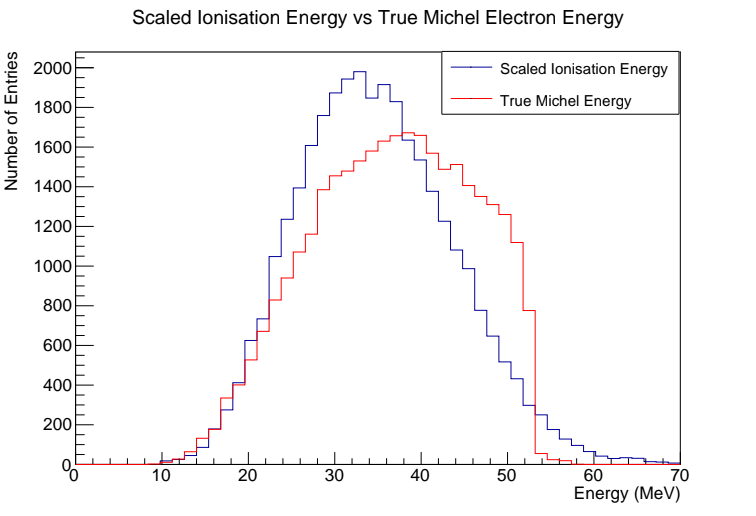
\includegraphics[width=\textwidth, height=0.68\textwidth]{figures/reco_v_mich.png}
	\caption
	[Reconstructed Energy vs True Michel Electron Energy.]
	{Reconstructed Energy vs True Michel Electron Energy.}
	\label{fig:reco_v_mich}
\end{figure}

\mccorrect{TODO: Energy resolution fits vs energy.}

The energy uncertainty and bias are estimated by fitting the fractional energy 
difference between the reconstructed and true Michel electron energies as a 
function of true Michel electron energy. The fractional energy difference, 
defined as 
\begin{equation}
	\Delta = \frac{E_{reco} - E_{true}}{E_{true}},
\end{equation}
is considered in bins of true Michel electron energy which are plotted in Figure
\ref{fig:frac_diff_energy}. This difference is fit with a gaussian distribution in each
bin in order to estimate the energy uncertainty and bias as a function of the 
true Michel electron energy.
\begin{figure}
	\centering
	% TODO: make set of fits as a function of energy
	\includegraphics[width=\textwidth, height=0.68\textwidth]{figures/frac_diff_v_energy.png}
	\caption
	[Fractional energy difference between reconstructed and true Michel electron
	energy.]
	{Fractional energy difference between reconstructed and true Michel electron
	energy.}
	\label{fig:frac_diff_energy}
\end{figure}

The energy resolution and bias as a function of true Michel electron energy are 
estimated as the standard deviation and mean of the gaussian fit to the
fractional energy difference in each energy bin, these values are plotted in
Figure \ref{fig:res_and_bias_energy}. \mccorrect{TODO: analysis of results}.
\begin{figure}
	\centering
	% TODO: make set of fits as a function of energy
	\includegraphics[width=\textwidth, height=0.68\textwidth]{figures/res_bias_v_energy.png}
	\caption
	[Energy resolution and bias as a function of true Michel electron energy.]
	{Energy resolution and bias as a function of true Michel electron energy.}
	\label{fig:res_and_bias_energy}
\end{figure}

\section{Conclusions} \label{ME_EU}
\begin{mccorrection}
	\begin{itemize}
		\item Reco energy scaling
		\item Uncertainty vs energy
		\item Differences in dune far detector
	\end{itemize}
\end{mccorrection}
